\newpage

\section{Testovanie}

Cieľom overovania bolo zistiť či algoritmus na odhaľovanie dlhodobých 
preferencií postavený na obdobiach dokáže poskytnúť lepšie výsledky ako 
agregácia hodnôt.

\paragraph{Vlastné testovanie}

Preto som sa rozhodol najskôr vytvoriť jedného testovacieho požívateľa a sledovať 
ako sa s časom bude menit účinnosť oboch algorimtov. 

Pri tomto testovaní sa porovnával používateľov zámer s niekoľkými odporučeniami algoritmov.
Zámer bol tvorený skupinou kapiel alebo typov dokumentov. Vzhľadom na unikátnosť piesní
sme sa rozhodoli nepoužiť pri testovani tento parameter.

Podobnosť užitočnosti odporúčaní sme hodnotili podľa toho, koľko kapiel a typov dokumentov
sa nachádza aj v zámere aj vo výsledku. Tento prístup je vyjadrený matematicky 
rovnicou \ref{eq:result_set_utility}.

\begin{equation}\label{eq:result_set_utility}
užitočnosť(R) = \frac{\sum\limit_{i=0}^{N}1 + \sum\limit_{i=0}^{M} 1 +\sum\limit_{i=0}^{K}1}{3}
\end{equation}

Rovnica obsahuje \(R\) čo je množina odporúčaní, \(N\), čo je počet piesni ktoré sú aj v
zámere aj v odporúčaní, \(M\) je počet interpretov, ktorí sú aj v zámere aj v odporučení a 
\(K\) je počet typov dokumentov, ktoré su tiež prienikom odporučení a zámeru.

Na obrázku \ref{fig:manual_testing_results} môžeme vidieť výsledok tohoto testu.

\begin{figure}
    \begin{center}
        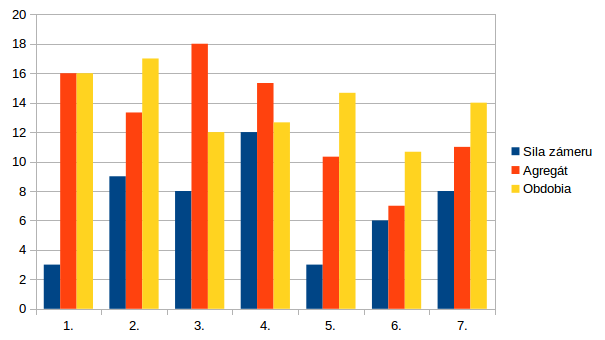
\includegraphics{manual_testing_results}
        \caption{Graf výsledkov pre manualny test}
        \label{fig:manual_testing_results}
    \end{center}
\end{figure}

Pokračovať v testoch nemalo zmysel vzhľadom na to, že agregačný algoritmus v predposlednom
aj v poslednom teste vrátil rovnaké výsledky. Čo vzhľadom na jeho povahu znamená, že 
menšie zámery už nemajú vplyv na jeho výsledok.

\subsection{Dotazník}

Ďaľšie testovanie prebehlo formov testovania aplikácie na webe pomocov respondentov, ktorý 
používali aplikáciu rôzne časove obdobia, následne sa im boli ponúknute odporúčania z obidvoch 
algoritmov a oni vyhodnotili ktorí im viacej vyhovuje. Na obrázku \ref{fig:dotaznik} môžeme 
vydieť výsledky dotazníku.

\begin{figure}
    \begin{center}
        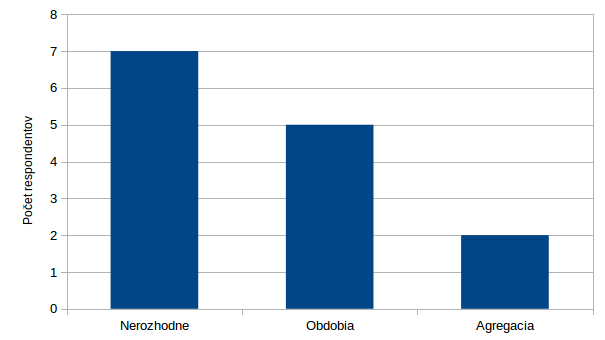
\includegraphics{dotaznik}
        \caption{Graf výsledkov pre dotazník}
        \label{fig:dotaznik}
    \end{center}
\end{figure}

Okrem tohoto porovnávania som ešte zisťoval či na stránke dokumentu používatelia viac preferovali
panel s podobnými dokumentamy alebo panel z odporúčaním na báze obdobý. Výsledky môžeme
vidieť na obrázku \ref{fig:dotaznik_podobnost}


\begin{figure}
    \begin{center}
        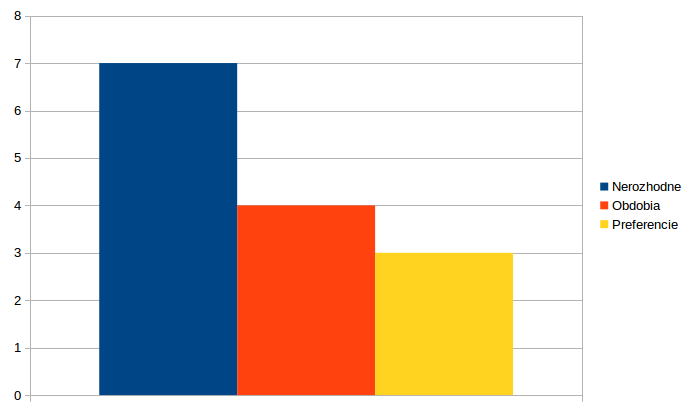
\includegraphics[scale=0.80]{dotaznik_podobnost}
        \caption{Graf výsledkov pre dotazník}
        \label{fig:dotaznik_podobnost}
    \end{center}
\end{figure}
